\documentclass[a4paper,12pt,french] {article}

\usepackage[TD]{../../../Style}

\renewcommand{\baselinestretch}{1.2}

\usetikzlibrary{angles}
\usepackage{tkz-euclide}

\pagestyle{empty}
% Passage en A3
%\geometry{a3paper,landscape,bottom=7mm,twocolumn}
%\setlength{\headwidth}{39cm} %42cm-2*margin pour fancyhdr

\begin{document}

\compo
{
\begin{center}
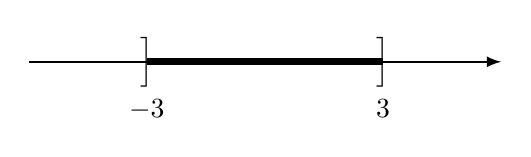
\begin{tikzpicture}[>=latex]
    \draw[thick,->] (0,0) --(6,0);
    \foreach \xp in {0.5,1,...,5.5}{\node[] at (\xp,0) {$\shortmid$};}
    \node[] at (4.5,0) {$\textbf{\Big]}$};
    \node[below=10pt] at (4.5,0) {$3$};
    \draw[line width=2.5pt] (1.5,0) --(4.5,0);
    \node[] at (1.5,0) {$\textbf{\Big]}$};
    \node[below=10pt] at (1.5,0) {$-3$};
\end{tikzpicture}
\end{center}
}
{
\begin{center}
\begin{tikzpicture}[>=latex]
    \draw[thick,->] (0,0) --(5,0);
    \foreach \xp in {0.5,1,...,4.5}{\node[] at (\xp,0) {$\shortmid$};}
    \node[below=10pt] at (1.5,0) {$0$};
    \node[stylepoint,fill=blue] at (3.14,0) {};
\end{tikzpicture}
\end{center}
}

\vfill

\compo
{
\begin{center}
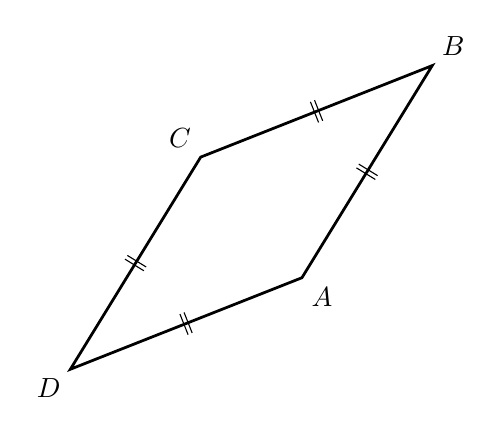
\begin{tikzpicture}[rotate=-50]
\coordinate[label=below right:$A$] (A) at (1,0);
\coordinate[label=above right:$B$] (B) at (0,3);
\coordinate[label=above left:$C$] (C) at (-1,0);
\coordinate[label=below left:$D$] (D) at (0,-3);
\draw[line width=1pt,cap=round] (A) -- (B) -- (C) -- (D) -- (A) -- cycle;
\tkzMarkSegment[pos=0.5,mark=||](A,B) 
\tkzMarkSegment[pos=0.5,mark=||](B,C) 
\tkzMarkSegment[pos=0.5,mark=||](C,D) 
\tkzMarkSegment[pos=0.5,mark=||](D,A) 
\end{tikzpicture}
\end{center}
}
{
\begin{center}
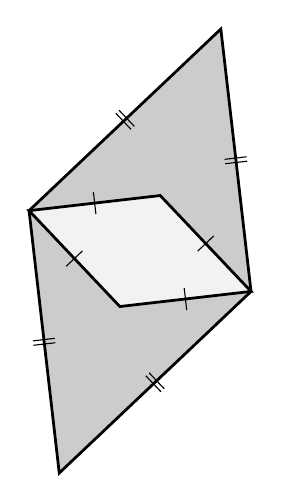
\begin{tikzpicture}[rotate=-20]
\coordinate (A) at (1.5,0);
\coordinate (B) at (0,3);
\coordinate (C) at (-1.5,0);
\coordinate (D) at (0,-3);
\coordinate (E) at (0,0.75);
\coordinate (F) at (0,-0.75);

\draw[line width=1pt,cap=round,fill=black!20] (A) -- (B) -- (C) -- (D) -- (A) -- cycle;
\draw[line width=1pt,cap=round,fill=black!5] (A) -- (E) -- (C) -- (F) -- (A) -- cycle;

\tkzMarkSegment[pos=0.5,mark=||](A,B) 
\tkzMarkSegment[pos=0.5,mark=||](B,C) 
\tkzMarkSegment[pos=0.5,mark=||](C,D) 
\tkzMarkSegment[pos=0.5,mark=||](D,A)

\tkzMarkSegment[pos=0.5,mark=|](A,E) 
\tkzMarkSegment[pos=0.5,mark=|](E,C) 
\tkzMarkSegment[pos=0.5,mark=|](C,F) 
\tkzMarkSegment[pos=0.5,mark=|](F,A)
\end{tikzpicture}
\end{center}
}

\vfill

\compo
{
\begin{center}
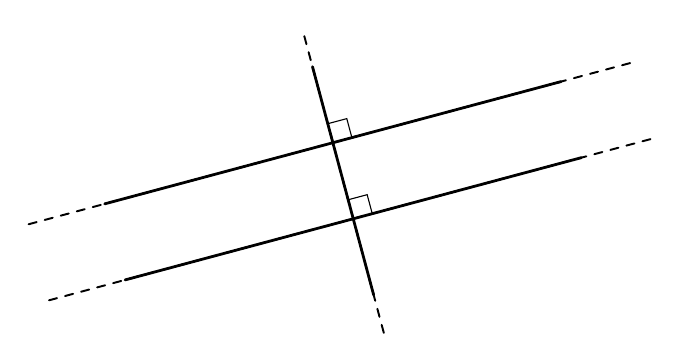
\begin{tikzpicture}[rotate=15]
\draw[line width=1pt,cap=round] (-3,0) -- (3,0);
\draw[line width=0.7pt,cap=round,dashed] (-4,0) -- (4,0);
\draw[line width=1pt,cap=round] (-3,1) -- (3,1);
\draw[line width=0.7pt,cap=round,dashed] (-4,1) -- (4,1);
\draw[line width=1pt,cap=round] (0,-1) -- (0,2);
\draw[line width=0.7pt,cap=round,dashed] (0,-1.5) -- (0,2.5);
\draw (0,0.25) -| (0.25,0);
\draw (0,1.25) -| (0.25,1);
\end{tikzpicture}
\end{center}
}
{
\begin{center}
\begin{tikzpicture}[rotate=15]
\draw[line width=1pt,cap=round] (-3,0) -- (3,0);
\draw[line width=0.7pt,cap=round,dashed] (-4,0) -- (4,0);
\draw[line width=1pt,cap=round] (0,-1) -- (0,1);
\draw[line width=0.7pt,cap=round,dashed] (0,-1.5) -- (0,1.5);
\draw (0,0.25) -| (0.25,0);
\end{tikzpicture}
\end{center}
}

\vfill

\compo
{
\begin{center}
\begin{tikzpicture}
\tkzInit[xmin=-1.5,xmax=3,ymin=-1.5,ymax=3]
\tkzSetUpAxis[ticka=3.5pt,tickb=3.5pt]	%Taille graduations
\tkzDrawX[]	%Axe X,pas de nombres,pas de flèche
\tkzDrawY[]	%Axe Y
\node[stylepoint,fill=blue] at (2,1) {};
\end{tikzpicture}
\end{center}
}
{
\begin{center}
\begin{tikzpicture}
\tkzInit[xmin=-1.5,xmax=4,ymin=-1.5,ymax=3]
\tkzSetUpAxis[ticka=3.5pt,tickb=3.5pt]	%Taille graduations
\tkzDrawX[]	%Axe X,pas de nombres,pas de flèche
\tkzDrawY[]	%Axe Y
\draw[stylevecteur] (0,0) -- (3,1);
\end{tikzpicture}
\end{center}
}

\vfill

\compo
{
\begin{center}
\begin{tikzpicture}
\tkzTabInit[lgt=1.4,espcl=1.5]{$x$/1, $f(x)$/1}{,,}
\tkzTabLine{,+,z,-,}
\end{tikzpicture}
\end{center}
}
{
\begin{center}
\begin{tikzpicture}
\tkzTabInit[lgt=1.4,espcl=1.5]{$x$/1, $f(x)$/1}{,,}
\tkzTabVar{+/,-/,+/}
\end{tikzpicture}
\end{center}
}

\newpage

\compo
{
\begin{center}
\begin{tikzpicture}[rotate=15]
\draw[line width=1pt,cap=round] (0,0) circle (3);
\coordinate (A) at ({1.5*sqrt(2)},{1.5*sqrt(2)});
\coordinate (B) at (-3,0);
\coordinate (C) at (3,0);
\node[stylepoint,fill=blue] (O) at (0,0) {};
\draw[line width=1pt,cap=round] (A) -- (B) -- (C) -- (A) -- cycle pic[draw=black,angle radius=2.5mm,thin] {right angle=B--A--C};
\end{tikzpicture}
\end{center}
}
{
\begin{center}
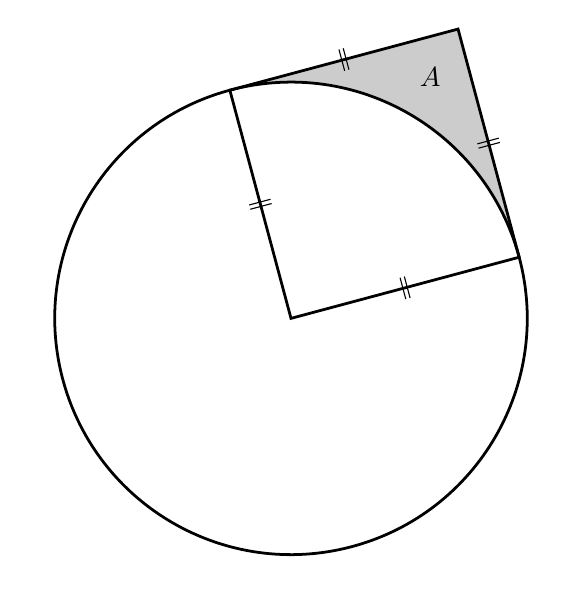
\begin{tikzpicture}[rotate=15]
\coordinate (A) at (0,0);
\coordinate (B) at (3,0);
\coordinate (C) at (3,3);
\coordinate (D) at (0,3);

\begin{scope}
\clip (A) -- (B) -- (C) -- (D) -- (A) -- cycle;
\fill[color=black!20,even odd rule] (A) -- (B) -- (C) -- (D) -- (A) -- cycle (0,0) circle (3);
\end{scope}

\draw[line width=1pt,cap=round] (0,0) circle (3);
\draw[line width=1pt,cap=round] (A) -- (B) -- (C) -- (D) -- (A) -- cycle;
\tkzMarkSegment[pos=0.5,mark=||](A,B)
\tkzMarkSegment[pos=0.5,mark=||](B,C)
\tkzMarkSegment[pos=0.5,mark=||](C,D)
\tkzMarkSegment[pos=0.5,mark=||](D,A)
\node at (2.5,2.5) {$\mathscr A$};
\end{tikzpicture}
\end{center}
}

\vfill

\compo
{
\begin{center}
\begin{tikzpicture}[scale=2,rotate=10]
\draw[stylevecteur] (0,0) -- (2,1) node[pos=0.5,above left] {$\vv u$};
\draw[stylevecteur] (2,1) -- (4,0) node[pos=0.5,above right] {$\vv v$};
\draw[stylevecteur,draw=red,line width=2pt] (0,0) -- (4,0) node[pos=0.5,below] {$\vv u + \vv v$};
\end{tikzpicture}
\end{center}
}
{
\begin{center}
\begin{tikzpicture}
\draw[stylevecteur] (-2,1) -- ++(4,2) node[pos=0.5,above left] {$\vv u$};
\draw[stylevecteur] (0,0) -- ++(4,2) node[pos=0.5,below right] {$\vv v = \vv u$};
\end{tikzpicture}
\end{center}
}

\vfill

\compo
{
\begin{center}
\begin{tikzpicture}[scale=1.5,rotate=10]
\coordinate[label=left:$A$] (A) at (-2,0);
\coordinate[label=right:$B$] (B) at (2,0);
\coordinate[label=above:$C$] (C) at (0,2);
\node[stylepoint,minimum size=0.5pt,fill=blue,inner sep=1pt] (O) at ($0.415*(C)$) {}; % A la main
\draw (A) -- (B) -- (C) -- (A) -- cycle;
\draw (O) circle ({sqrt(4*4*(2*sqrt(8)-4)/(4*(4+2*sqrt(8))))});
\end{tikzpicture}
\end{center}
}
{
\begin{center}
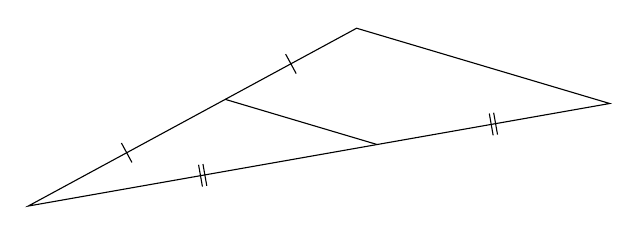
\begin{tikzpicture}[scale=1.5,rotate=10]
\coordinate (A) at (-3,0);
\coordinate (B) at (2,0);
\coordinate (C) at (0,1);
\coordinate (D) at ($0.4*(A)+0.6*(B)$);
\coordinate (E) at ($0.4*(A)+0.6*(C)$);
\draw (A) -- (B) -- (C) -- (A) -- cycle;
\draw (D) -- (E);
\tkzMarkSegment[pos=0.5,mark=||](A,D)
\tkzMarkSegment[pos=0.5,mark=||](D,B)
\tkzMarkSegment[pos=0.5,mark=|](A,E)
\tkzMarkSegment[pos=0.5,mark=|](E,C)
\end{tikzpicture}
\end{center}
}

\vfill

\compo
{
\begin{center}
\begin{tikzpicture}
\begin{axis}[
styleglobal,
width=0.9*\linewidth,
xmin=-3, xmax=6,
ymin=-1.5, ymax=4.5,
ytick distance=1,
xtick distance=1,
grid=none,
ticks=none,
]
\addplot[styleplot]{2} node [pos=0.9,above left] {$\mathscr C_f$};
\end{axis}
\end{tikzpicture}
\end{center}
}
{
\begin{center}
\begin{tikzpicture}
\begin{axis}[
styleglobal,
width=0.9*\linewidth,
xmin=-3, xmax=6,
ymin=-3, ymax=3,
ytick distance=1,
xtick distance=1,
grid=none,
ticks=none,
]
\addplot[styleplot]{2.5*sin(deg(2*x))} node [pos=0.8,above right] {$\mathscr C_f$};
\end{axis}
\end{tikzpicture}
\end{center}
}
\end{document}